\documentclass{article}
\usepackage[utf8]{inputenc}

\title{CPA Project}
\author{Erdogan Kevin, Katia Amichi}
\date{April 2019}

\usepackage{graphicx}
\usepackage{placeins}
\usepackage{hyperref}
\usepackage[noabbrev,capitalize]{cleveref}
\usepackage{natbib}


\begin{document}

\maketitle

\section{Handling a large graph}
Our setup for running times for this part and further is :
i5-7440HQ CPU @ 2.8GHz. \\
Git link to our code : \url{https://github.com/zeeer0/cpa_project}
\subsection{A special quantity}
The following results were provided by the function "specialQuantity()", we have first cleaned the graph file and then calculate the quantity.\\ \\
\begin{tabular}{ |p{3.7cm}||p{3.7cm}|p{3.7cm}|  }
 \hline
 \multicolumn{3}{|c|}{ Special Quantity } \\
 \hline
 Graph Name & $\mathcal{Q}_G$ & Running time(s)\\
 \hline
 Email-Eu-core & 88 109 182 & 0.003146\\
 Amazon & 103 415 531  & 0.1827 \\
 Live Journal & 789 000 450 609 & 4.820176\\
 Orkut & 22 292 678 512 329 & 15.769974\\
 Friendster & 379 856 554 324 947 & 474.847368\\
 \hline
\end{tabular}

\clearpage

\subsection{Degree distribution}
For this part, we have generated a file named "degreeDistribution.txt" thanks to the function "degreeDistribution()" for each graph and then plot it with gnuplot to have the following results.\\ \\
\begin{figure}[h!]
  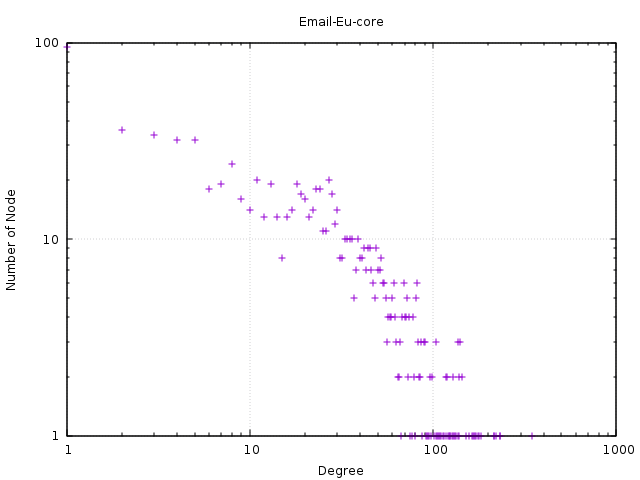
\includegraphics[width=12cm, height=6cm]{email.png}
  \caption{Degree distribution for Email-Eu-Core}
\end{figure}
\FloatBarrier
\begin{figure}[h!]
  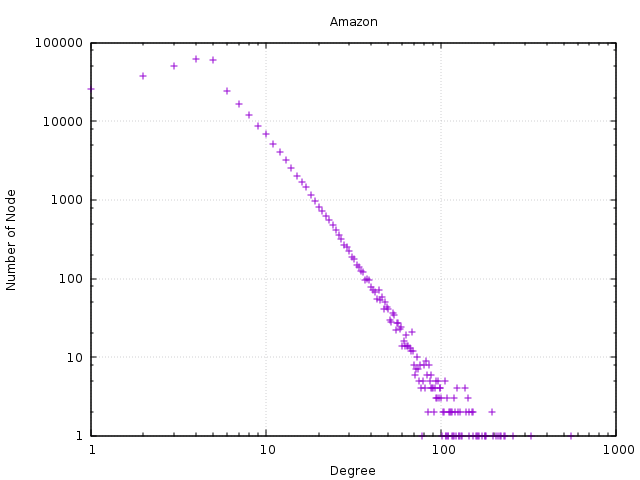
\includegraphics[width=12cm, height=7cm]{amazon.png}
  \caption{Degree distribution for Amazon}
\end{figure}
\FloatBarrier
\begin{figure}[h!]
  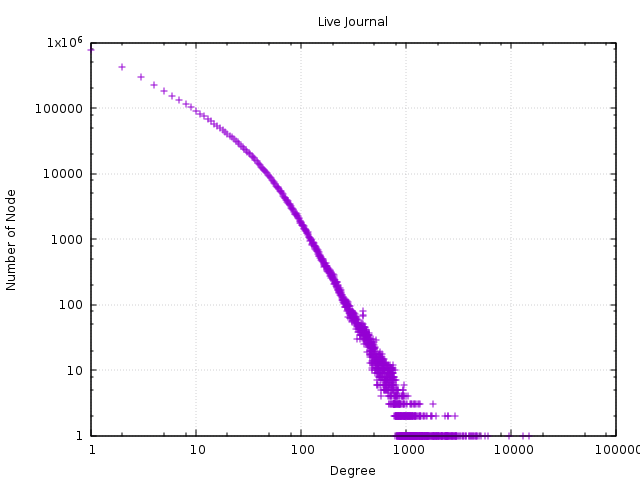
\includegraphics[width=12cm, height=7cm]{live_journal.png}
  \caption{Degree distribution for Live Journal}
\end{figure}
\FloatBarrier
\begin{figure}[h!]
  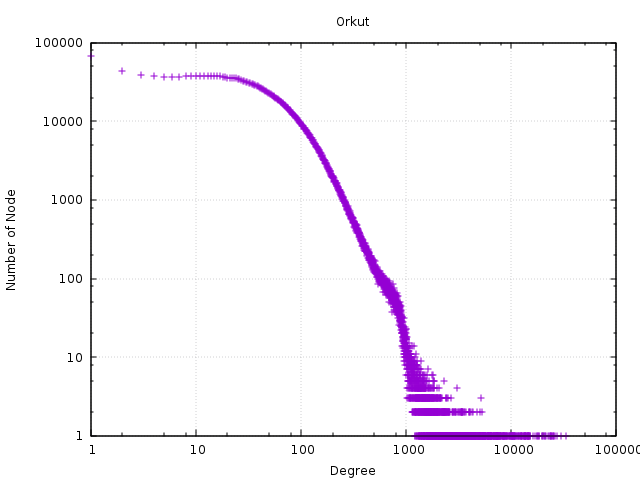
\includegraphics[width=12cm, height=8cm]{orkut.png}
  \caption{Degree distribution for Orkut}
\end{figure}
\FloatBarrier
\begin{figure}[h!]
  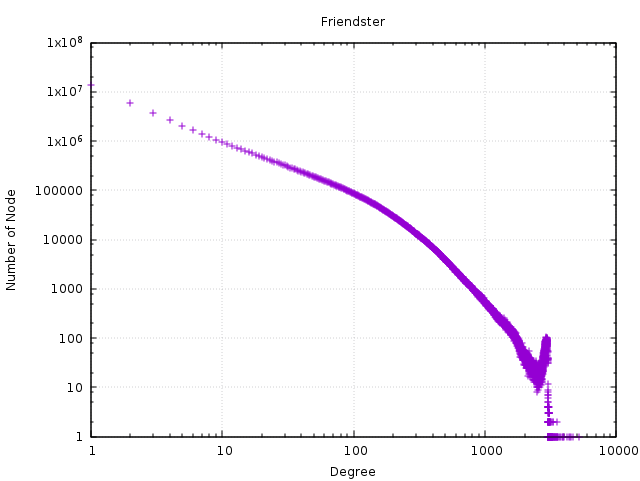
\includegraphics[width=12cm, height=8cm]{friendster.png}
  \caption{Degree distribution for Friendster}
\end{figure}
\FloatBarrier

\subsection{Three graph datastructures}
Firstly, for the List of Edge datastructure, it is a simple way to store a graph in memory but very not efficient for the search of neighbours.\\ Amount of memory required : $sizeof(int)$ x 2 x $NumberOfEdges$ bytes.\\
For example, Friendster has 1 806 067 135 edges, so we need 14.5 Gig of RAM for storing the graph in memory.\\ \\
Secondly, for the Adjacency Matrix datastructure, we have access to neighbours of a node very quickly but the required amount of memory for storing the graph fastly becomes creepy.\\ Amount of memory required : $sizeof(int)$ x $NumberOfNodes^{2}$ bytes.\\
In our example, we need up to 17 217 830 Gig of RAM... \\ \\
And finally, for the Adjacency Array datastructure, it is the best way of the three datastructures for storing a huge graph because we need (approximately) the same amount of memory as the List of Edge datastructure but we have a very simple and efficient way to access to the neighbours of a node.\\ Amount of memory required : $sizeof(int)$ x 2 x $NumberOfEdges$ + $C$ bytes, where $C$ is a negligible amount of memory.

\clearpage

\subsection{Breadth-First Search}
For this exercise, we could not run the program on Friendster graph because it requires at least 16Gig of free RAM to store it in memory.\\
The results were provided by the function "max connections diameter()".\\ \\
\begin{tabular}{ |p{3.7cm}||p{3.7cm}|p{3.7cm}|  }
 \hline
 \multicolumn{3}{|c|}{ Listing Triangles } \\
 \hline
 Graph Name & Fraction of Nodes in the largest connected component & Lower Bound\\
 \hline
 Email-Eu-core & 986 & 7 \\
 Amazon & 334863 & 47\\
 Live Journal & 3997962 & 21\\
 Orkut & 3072441 & 9 \\
 Friendster & null & null\\
 \hline
\end{tabular}

\subsection{Listing triangles}
For Friendster graph, same as above.\\
The results are given by the function "numberOfTriangle()", they are calculated by storing the graph in a Adjacency Array datastructure.\\ \\
\begin{tabular}{ |p{3.7cm}||p{3.7cm}|p{3.7cm}|  }
 \hline
 \multicolumn{3}{|c|}{ Listing Triangles } \\
 \hline
 Graph Name & Number of Triangles & Running time\\
 \hline
 Email-Eu-core & 105 461 & 0.012474\\
 Amazon & 667 129 & 0.129404 \\
 Live Journal & 177 820 130 & 36.073947\\
 Orkut & 627 584 181 & 392.643731\\
 Friendster & null  & null\\
 \hline
\end{tabular}

\clearpage

\section{Practical Work - Community Detection}
\subsection{Simple Benchmark}

\textbf{With p=0.6 and q=0.001}
\begin{figure}[h!]
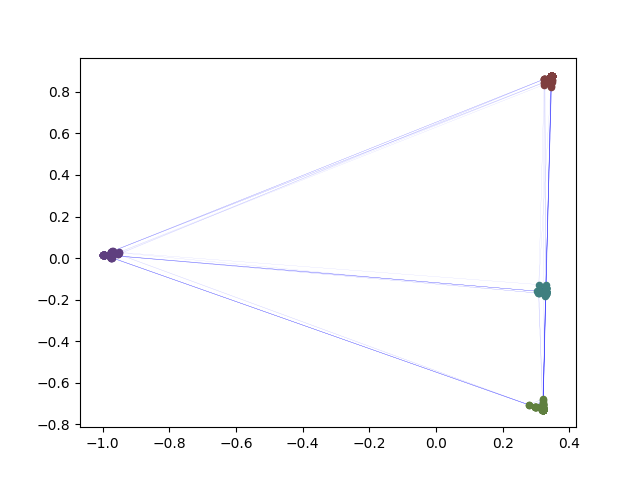
\includegraphics[width=12cm, height=7cm]{Figure_1.png}
  \caption{Graphs with various values of p and q}
\end{figure}
\FloatBarrier

\textbf{With p=0.6 and q=0.1}
\begin{figure}[h!]
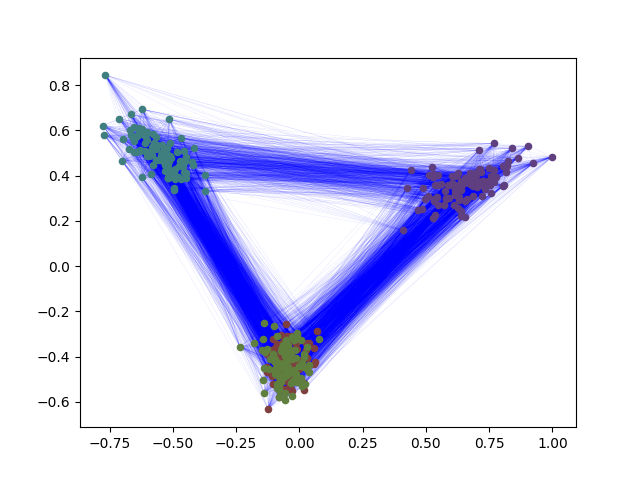
\includegraphics[width=12cm, height=7cm]{Figure_2.png}
  \caption{Graphs with various values of p and q}
\end{figure}
\FloatBarrier

\textbf{With p=0.6 and q=0.7}
\begin{figure}[h!]
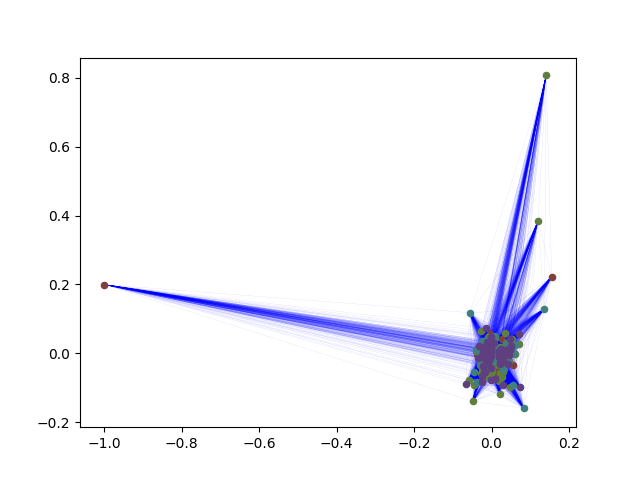
\includegraphics[width=12cm, height=7cm]{Figure_3.png}
  \caption{Graphs with various values of p and q}
\end{figure}
\FloatBarrier

We notice that the more we diminish the value of q, the more we can distinguish the communities, as we can see on the different plots, when we increase the value of q we can see the separation between the communities.

\clearpage

\subsection{Label propagation}

\begin{figure}[h!]
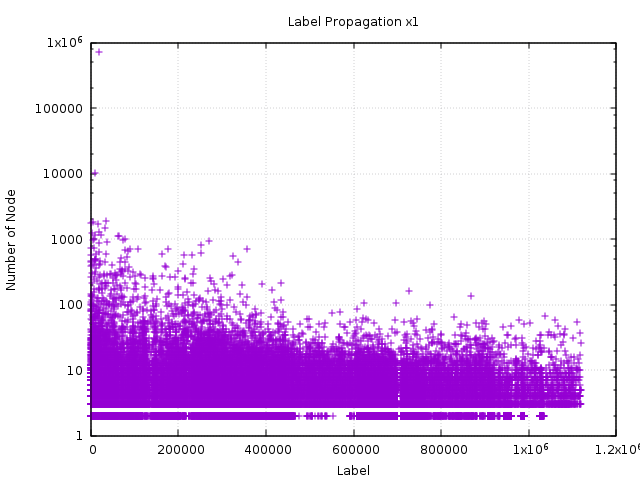
\includegraphics[width=12cm, height=7cm]{labelPropagationx1.png}
  \caption{\label{fig:histoSize}Histogram of the sizes of the communities}
\end{figure}
\FloatBarrier

\begin{figure}[h!]
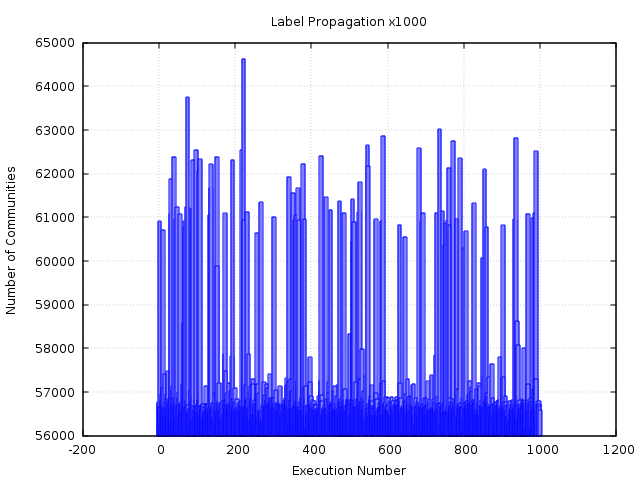
\includegraphics[width=12cm, height=7cm]{labelPropagationx1000.png}
  \caption{\label{fig:histoNum}Histogram of the numbers of communities}
\end{figure}
\FloatBarrier

For the \cref{fig:histoSize}, we can see a large amount of communities but they are, for the most, not exceeding 100 nodes.\\
More over in \cref{fig:histoNum}, thanks to the random shuffling, we have each time another amount of communities for each execution. But we can see that there is a range which is [55000:65000] that the number of communities stays in.


\section{Practical Work - Pagerank}
\subsection{PageRank (directed graph)}
\subsubsection{Convergence}
\begin{figure}[h!]
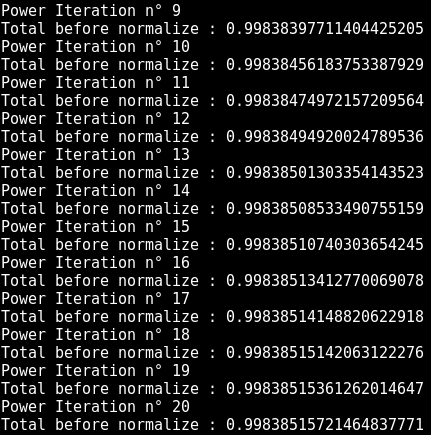
\includegraphics[width=11cm, height=6.5cm]{powerIter.png}
 
  \caption{ \label{fig:iterations} Number of iterations to reach convergence}
\end{figure}
\FloatBarrier

As we see in \cref{fig:iterations}, we reached convergence after about 15 iterations with $\alpha$ = 0.15.
\subsubsection{Pagerank Results}
For this part, we have implemented the algorithm of Power Iteration and run it 20 times to get the following results.\\ \\
\begin{tabular}{ |p{1cm}||p{4.5cm}|p{5.5cm}|  }
 \hline
 \multicolumn{3}{|c|}{ Highest and Lowest Pagerank } \\
 \hline
 Place & Highest Pagerank & LowerPageRank\\
 \hline
 1 & United States & Aberdeen (disambiguation) \\
 2 & United Kingdom  &  Animal (disambiguation) \\
 3 & Germany & Antigua and Barbuda \\
 4 & 2007 & AWK (disambiguation) \\
 5 & 2006 & Demographics of American Samoa \\
 \hline
\end{tabular}

\clearpage

\subsection{Correlations}
\begin{figure}[h!]
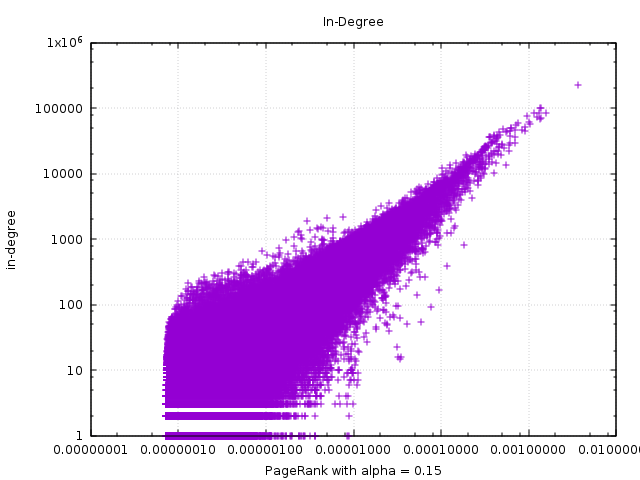
\includegraphics[width=12cm, height=7cm]{in_degree.png}
  \caption{Scatter plot with y = in-degree}
\end{figure}
\FloatBarrier
\begin{figure}[h!]
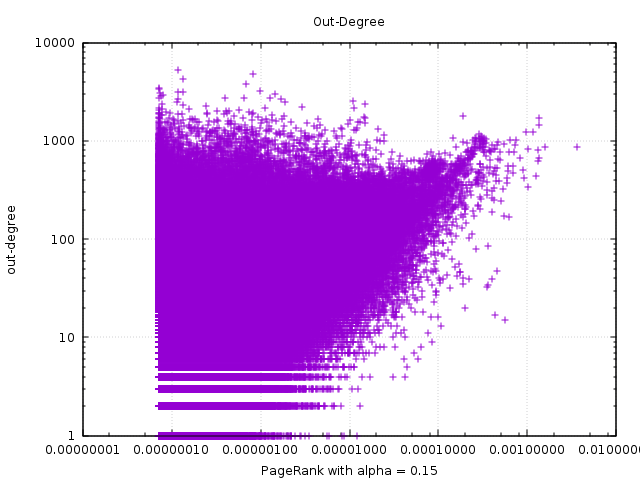
\includegraphics[width=12cm, height=7cm]{out_degree.png}
  \caption{Scatter plot with y = out-degree}
\end{figure}
\FloatBarrier
\begin{figure}[h!]
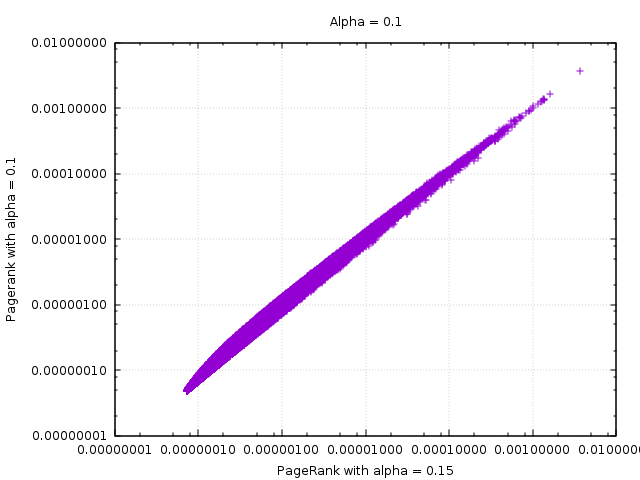
\includegraphics[width=12cm, height=7cm]{correlationPart3.png}
  \caption{Scatter plot with y = Pagerank with $\alpha$ = 0.1}
\end{figure}
\FloatBarrier
\begin{figure}[h!]
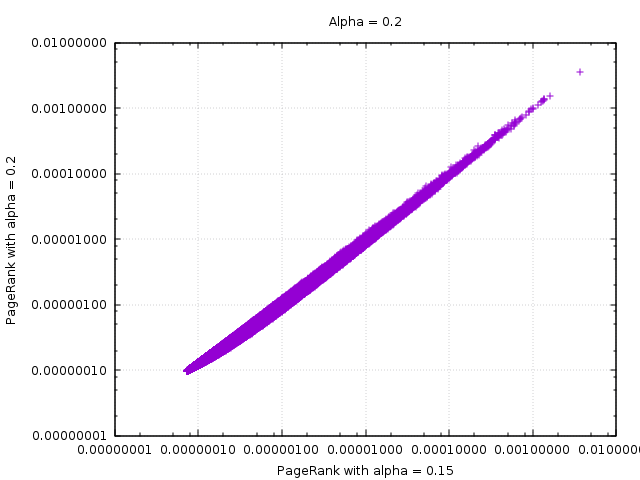
\includegraphics[width=12cm, height=7cm]{correlationPart4.png}
  \caption{Scatter plot with y = Pagerank with $\alpha$ = 0.2}
\end{figure}
\FloatBarrier
\begin{figure}[h!]
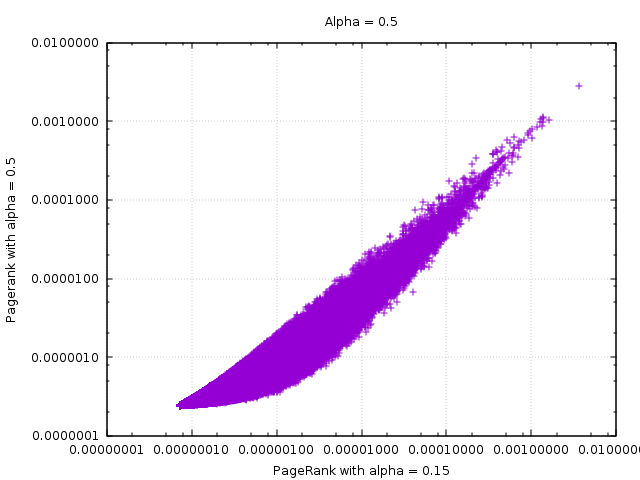
\includegraphics[width=12cm, height=7cm]{correlationPart5.png}
  \caption{Scatter plot with y = Pagerank with $\alpha$ = 0.5}
\end{figure}
\FloatBarrier
\begin{figure}[h!]
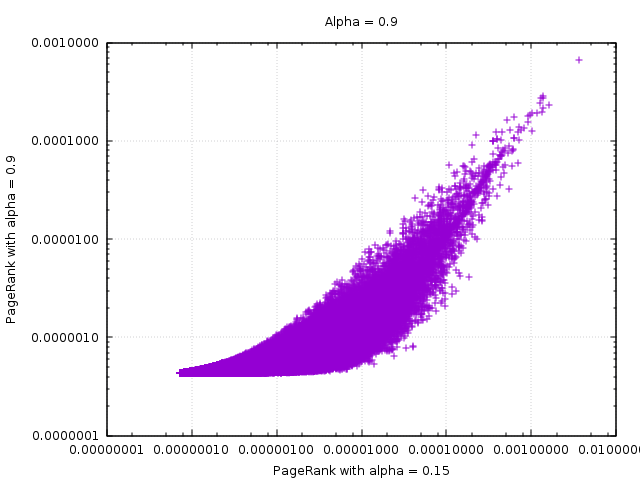
\includegraphics[width=12cm, height=7cm]{correlationPart6.png}
  \caption{Scatter plot with y = Pagerank with $\alpha$ = 0.9}
\end{figure}
\FloatBarrier

\clearpage

 \subsubsection{Response}
We used log scales because the Pageranks were too small.\\
About correlations, when $\alpha_1$ and $\alpha_2$ are close in x-axis and y-axis, it seems to be a linear function (Pageranks are very similar) but when $\alpha_2$ in y-axis increase, the Pageranks in y-axis seems to be lower.

\section{Densest subgraph}
\subsection{k-core decomposition}

\begin{tabular}{ |p{2.5cm}||p{1.5cm}|p{2.8cm}|p{2.8cm}|p{2.8cm}| }
 \hline
 File & Core & The average degree density & The edge density & The size of a densest core ordering prefix\\
 \hline
 Email-Eu-core & 34 & 27.352942 & 0.147059 & 187\\
 Amazon & 6 & 3.684211 & 0.204678 & 19 \\
 Live Journal & 360 & 189.463547 & 0.494683 & 384\\
 Orkut & 259 & 227.834030 & 0.008583 & 26546\\
 Friendster & null & null & null & null\\
 \hline
\end{tabular}


\subsection{Graph mining with k-core}
We notice that there is a group of authors who have a core of 14 and who do not have a high degree and that all its author are of the same nationality.

\begin{figure}[h!]
  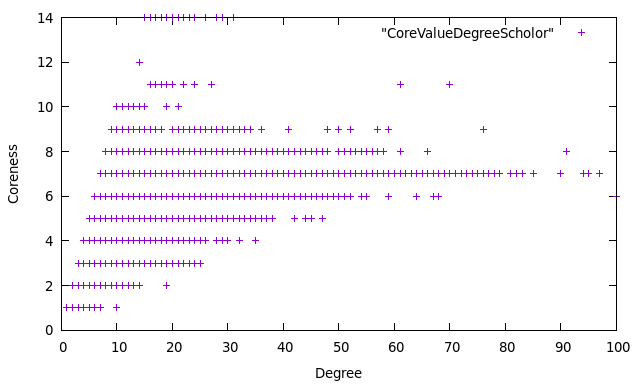
\includegraphics[width=12cm, height=7cm]{google_scholor.png}
  \caption{Core Value Degree for Scholor}
\end{figure}

With the logarithmic scales we notice that there is
a limit that does not exceed.
\begin{figure}[h!]
  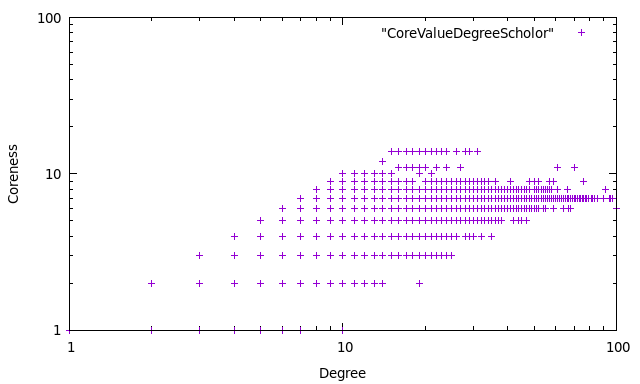
\includegraphics[width=12cm, height=7cm]{CPlotlog.png}
  \caption{Core Value Degree for Scholor Log}
\end{figure}

We get the following results : 

\begin{itemize}
    \item k-core: 14
    \item Average degree density = 9.84719
    \item Edge density = 0.94215
    \item Size of a core ordering prefix = 28
\end{itemize}

\textbf{The authors :}
They are authors who are quoted a lot between them.
Sa-kwang, Sung-Pil, Chang-Hoo, Yun-soo, Hong-Woo, Jinhyung, Hanmin, Do-Heon, Myunggwon,
Won-Kyung, Hwamook, Minho, Won-Goo, Jung, Dongmin, Mi-Nyeong, Sung, Minhee, Sungho,
Seungwoo, Heekwan, Jinhee, Taehong, Mikyoung ,Ha-neul ,Seungkyun, Yun-ji.


\subsection{Densest subgraph}
We note that the more we increase the number of iteration, the closer we get to the values obtained on the first exercise.

\subsubsection{t = 10}
\begin{tabular}{ |p{3.0cm}||p{3.0cm}|p{3.0cm}|p{3.0cm}| }
 \hline
 \multicolumn{4}{|c|}{ The number of iterations t to 10 } \\
 \hline
 File & The average degree density & The edge density & The size of a densest core ordering prefix\\
 \hline
 Email-Eu-core & 28.0629 & 2.30952 & 70\\
 Amazon & 4.8850 & 0.01888 & 244 \\
 Live Journal & 199.8502 & 0.243066 & 232\\
 Orkut & 249.980 & 0.0587221 & 397\\
 \hline
\end{tabular}

\subsubsection{t = 100}
\begin{tabular}{ |p{3.0cm}||p{3.0cm}|p{3.0cm}|p{3.0cm}| }
 \hline
 \multicolumn{4}{|c|}{ The number of iterations t to 100 } \\
 \hline
 File & The average degree density & The edge density & The size of a densest core ordering prefix\\
 \hline
 Email-Eu-core & 27.0995 & 2.30952 & 185\\
 Amazon & 4.7760 & 0.0998711 & 107 \\
 Live Journal & 191.082 & 0.243066 & 382\\
 Orkut & 228.827 & 0.0541537 & 1384\\
 \hline
\end{tabular}

\subsubsection{t = 1000}
\begin{tabular}{ |p{3.0cm}||p{3.0cm}|p{3.0cm}|p{3.0cm}| }
 \hline
 \multicolumn{4}{|c|}{ The number of iterations t to 1000 } \\
 \hline
 File & The average degree density & The edge density & The size of a densest core ordering prefix\\
 \hline
 Email-Eu-core & 27.4493 & 0.241783 & 229\\
 Amazon & 4.7760 & 0.0998711 & 98 \\
 Live Journal & 4.7556 & 0.0984641 & 441\\
 Orkut & nul &l null & null\\
 \hline
\end{tabular}

For 1000 iterations, it does not end in reasonable time.
    

We consider the dense subgraph problem that extracts a subgraph with a prescribed number of vertices that has the maximum number of edges in a given graph. 

Assuming that the density of the optimal output subgraph is high, where density is the ratio of number of edges to the number of edges in the clique on the same number of vertices, with proving that 2 * density score increases the max degree of the graph.


\subsection{Graph not fitting in main memory}
For this exercise, we implemented the same algorithm as Exercise 3 but each time running the file without storing it.
Although we keep nothing in memory, the slowest part is the file reading (which we do several times).

\end{document}
